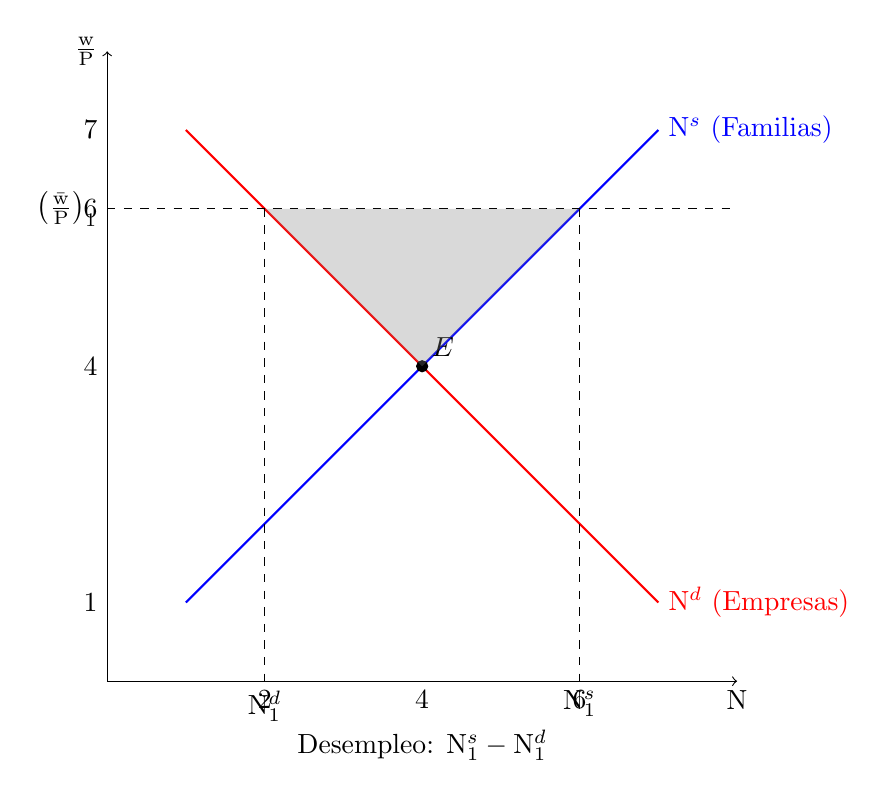
\begin{tikzpicture}
% Ejes
\draw[->] (0,0) -- (8,0) node[below] {$\mathrm{N}$}; % Eje horizontal (Cantidad de trabajo)
\draw[->] (0,0) -- (0,8) node[left] {$\frac{\mathrm{w}}{\mathrm{P}}$}; % Eje vertical (Salario real)
% Curva de oferta de trabajo (N^s): pendiente positiva
\draw[thick, blue] (1,1) -- (7,7) node[right] {$\mathrm{N}^s$ (Familias)};
% Curva de demanda de trabajo (N^d): pendiente negativa
\draw[thick, red] (1,7) -- (7,1) node[right] {$\mathrm{N}^d$ (Empresas)};
% Salario mínimo que genera desequilibrio (w/P = 6)
\draw[dashed] (0,6) node[left] {$\left(\frac{\bar{\mathrm{w}}}{\mathrm{P}}\right)_1$} -- (8,6);
% Puntos de oferta y demanda en el salario mínimo
\draw[dashed] (2,6) -- (2,0) node[below] {$\mathrm{N}^d_1$}; % Demanda
\draw[dashed] (6,6) -- (6,0) node[below] {$\mathrm{N}^s_1$}; % Oferta
% Punto de intersección teórico (equilibrio sin salario mínimo)
\draw[fill=black] (4,4) circle (2pt) node[above right] {$E$}; % Intersección N^s y N^d
% Área triangular sombreada (por debajo del salario mínimo, entre N^s y N^d)
\fill[gray, opacity=0.3] (2,6) -- (4,4) -- (6,6) -- cycle;
% Etiqueta de desempleo
\node[below, align=center] at (4,-0.5) {Desempleo: $\mathrm{N}^s_1 - \mathrm{N}^d_1$};
% Marcas en los ejes
\draw (0,1) node[left] {$1$};
\draw (0,4) node[left] {$4$};
\draw (0,6) node[left] {$6$};
\draw (0,7) node[left] {$7$};
\draw (2,0) node[below] {$2$};
\draw (4,0) node[below] {$4$};
\draw (6,0) node[below] {$6$};
\end{tikzpicture}
